\section{Evaluation}
\label{sec:Evaluation}
\subsection{Weaknesses}
\label{sec:Weaknesses}
\subsubsection{Masks}
\label{sec:MasksWeaknesses}

\begin{figure*}
\centering
\begin{minipage}{0.33\textwidth}
\centering
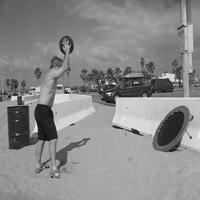
\includegraphics[width=2in]{frame_0074.jpg}
\caption{first figure}
\end{minipage}\hfill
\begin{minipage}{0.33\textwidth}
\centering
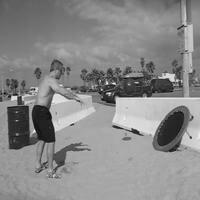
\includegraphics[width=2in]{frame_0076.jpg}
\caption{second figure}
\end{minipage}
\begin{minipage}{0.33\textwidth}
\centering
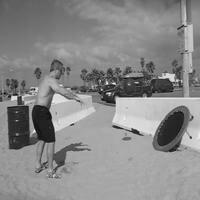
\includegraphics[width=2in]{frame_0076.jpg}
\caption{third figure}
\end{minipage}
\end{figure*}

Because of the way that masks are calculated (either as the median or the mean of the pixel values throughout the video), some type of ``interesting'' movement may be classified as part of the background. Consider Figure x which is a frame from a video of a man throwing a ball against a trampoline. The man's arms and the ball change position in almost every frame of the video. Because of this, it is easy for a median or average mask to isolate his arms and the ball. However, The man's torso (especially his upper legs) stay in almost exactly the same position throughout but constitute part of the interesting region in every frame of the video loop. This means that a median or average mask incorrectly classify those regions as part of the background. Figure x is a frame of a video where the a median mask has filtered out the background (by converting the pixels to black). It is easy to see that the man's legs are completely lost in the background. For these videos it is hard to apply masks in a coherent way. 
